\chapter{Experiment Setup} \label{ch:exp}

This chapter introduces the experiments designed to obtain the surrogate plant model and the correlations among input-output signals. After discussing the data visualization and pre-processing in Section \ref{ch:exp:data}, Section \ref{ch:exp:exp} describes in detail the experiments investigating the effects of varying numerous parameters on model performance; from these experiments the best-performing surrogate model is obtained. The outcome of these experiments and the metrics with which the model performance is evaluated are presented in Section \ref{ch:exp:results}. 

\section{First Glimpse at the Data} \label{ch:exp:data}

During the optical fiber drawing process described in Section \ref{ch:intro:fiber}, the industrial computer on the manufacturing plant records real-time data and logs them into (considerably large) CSV files. Each file contains week-long, timestamped data of measured BFD, tension, furnace power, capstan speed and acceleration, preform speed, helium tube temperature, controller's on/off status, among many others. A visualization of their typical values\footnote{Selected from Week 14, Subbatch 19 in Tower 48 training data.} is depicted in Figure \ref{fig:example_values}, and the range of each input is shown in Figure \ref{fig:values_hist}.

\begin{figure}[hp!]
    \centering
    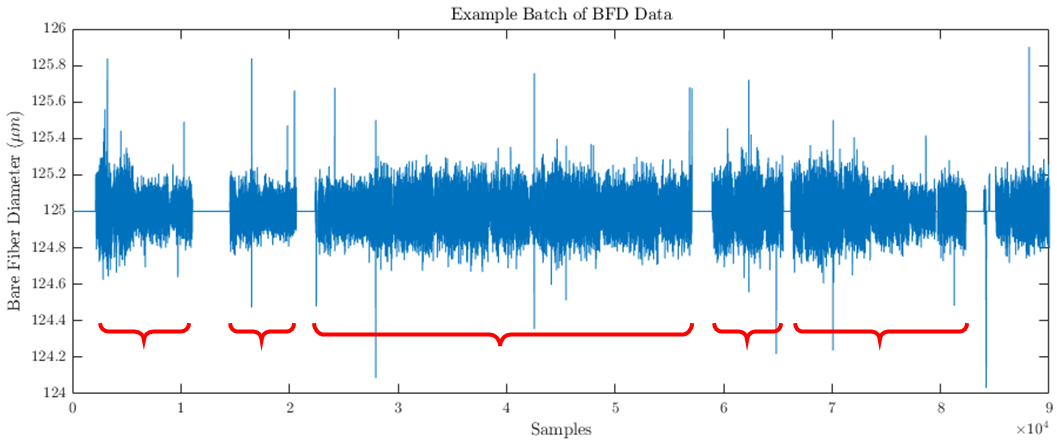
\includegraphics[width=0.8\textwidth]{figures/example_bfd2.png}
    \caption{A portion of the measured BFD signal in a week's data. Each subbatch is labeled with red curly braces.}
    \label{fig:example_bfd}
    
    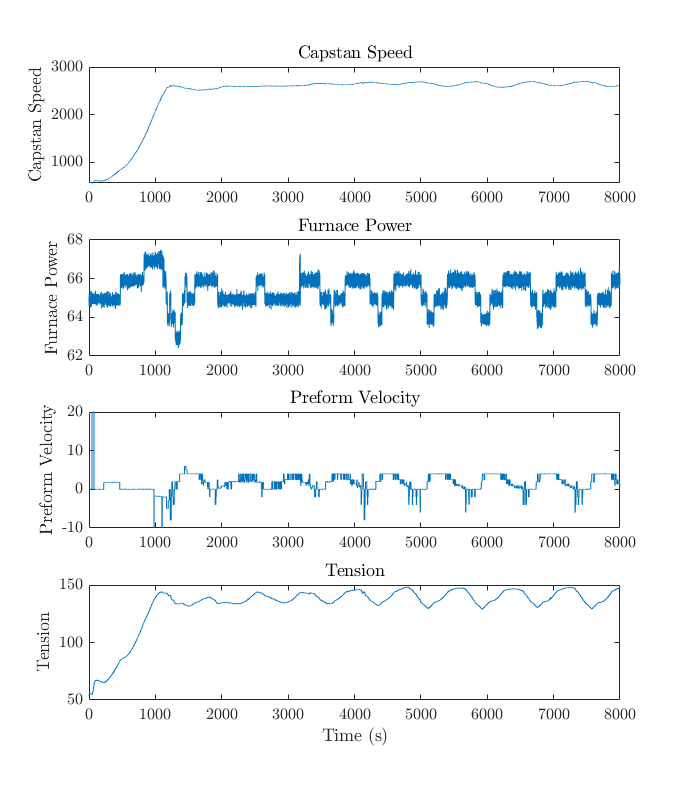
\includegraphics[width=0.85\textwidth]{figures/values.png}
    \caption{An example of input signals to the neural network in a particular subbatch.}
    \label{fig:example_values}
\end{figure}

\begin{figure}[t!]
    \centering
    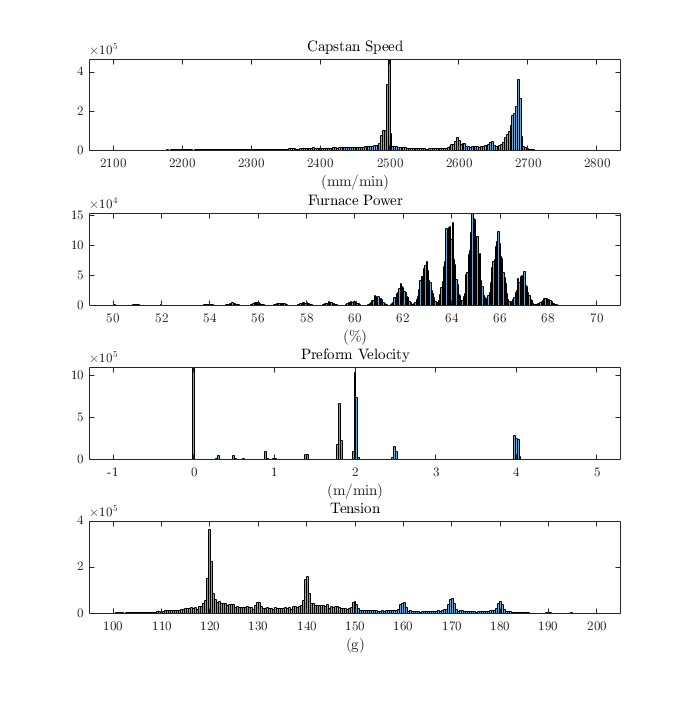
\includegraphics[width=\textwidth]{figures/values_hist.png}
    \caption{Histogram illustrating range of all input signals.}
    \label{fig:values_hist}
\end{figure}

Figure \ref{fig:example_bfd} illustrates a portion of the measured BFD signal in a typical week of production data. Per industrial standards, the nominal BFD is set at 125 microns ($\mu m$) to be compliant with general specifications for optical fiber. However, there are notable breaks in the fiber and perturbations for which the BFD diverges from target value. This is a normal part of the manufacturing process; breaks could occur due to underheating, coating defects, and other irregularities in the preform material \cite{breaks1, breaks2}. Manual intervention is required when this happens; the operator would manually disengage the controller, adjust the tower before re-engaging the controller to bring production back to nominal. 

Upon a closer look at each contiguous region of the BFD, stable production usually results in BFD measurements ranging from 124 to 126 microns. (Refer to Figure \ref{fig:example_bfd}.) In our analysis, we define each week of data as a \emph{batch}. Within a week, each contiguous region of stable production that are greater than 2000 samples is referred to as a \emph{subbatch}, illustrated with red curly braces in Figure \ref{fig:example_bfd}. Each subbatch is limited to a maximum length of 8000 samples to normalize the input size to the neural network. 

The main goal of the machine learning experiments is obtain a dynamical model, in the form of a neural network, that authentically represents the behavior of the aggregate fiber drawing plant. The developed surrogate model could be tested using classical methods (e.g. observing its frequency response) in simulation. Factors that impact the learning of said dynamical model include the neural network architecture, filter lengths, and steady-state range thresholds. We performed experiments investigating the effect of each of these factors on model performance, and from the experimental outcomes, we obtain the best-performing model to be used in a closed-loop simulation. 

\section{Learning Experiments and Explorations} \label{ch:exp:exp}

\subsection{Architecture Experiments} \label{ch:exp:arch}

In setting up the LSTM networks to represent the surrogate model of the plant, the inputs and outputs of the LSTM correspond to those of the black-boxed plant system in the schematics. Namely, the input variables are furnace power, helium tube temperature, capstan speed, and preform velocity; the output variables are the BFD and tension. Refer to the arrows into and out of the red dashed box in Fig. \ref{fig:stl_system_diag}.

We experimented with four different LSTM architecture designs: a single LSTM layer network, a single biLSTM layer network, a 3 side-by-side LSTM layer network, and a 3-layer deep LSTM network. In their architectures, the first layer is a normalization layer in which the inputs are subtracted by the mean and normalized by the standard deviation. It has been demonstrated that normalization of input data usually translates to numerical stability as well as better learning results \cite{normalization1, normalization2}. The first two architectures utilized a 128-neuron LSTM layer followed by a fully connected layer for output. Inspired by the results from \cite{gonzalez}, the side-by-side architecture sent its input to all of its three 128-neuron LSTM layers, concatenated their response, and passed it into a fully connected layer for output. The deep LSTM architecture has three 128-neuron LSTM layers stacked one after another. An illustration depicting these network architectures is shown in Fig. \ref{fig:nn_archs}. 

\begin{figure}[t!]
    \centering
    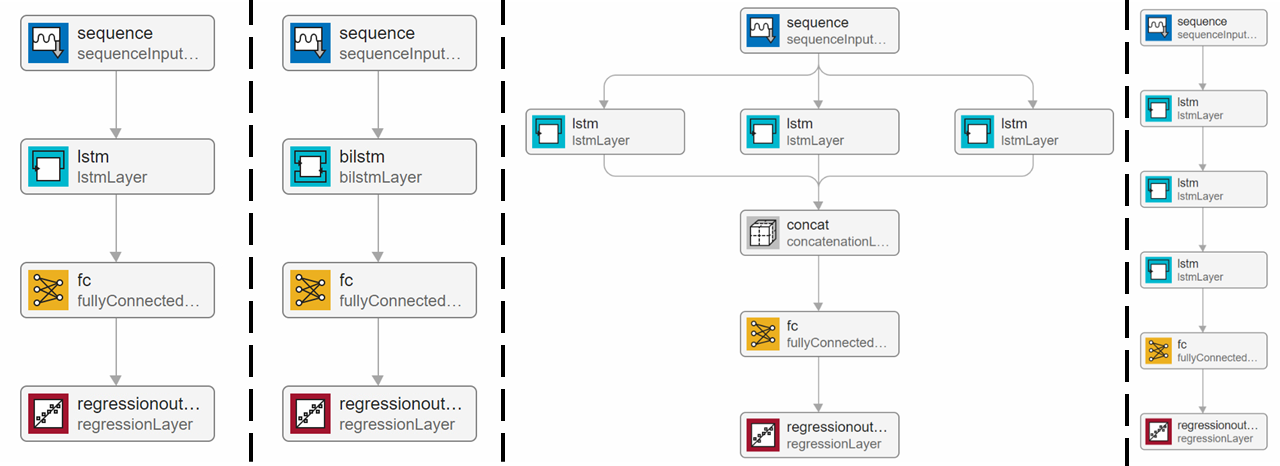
\includegraphics[width=\textwidth]{figures/architectures.png}
    \caption{Four architecture designs experimented in this paper: single layer LSTM, single layer biLSTM, side-by-side LSTM, deep LSTM (from left to right, respectively). }
    \label{fig:nn_archs}
\end{figure}

\begin{figure}[t!]
    \centering
    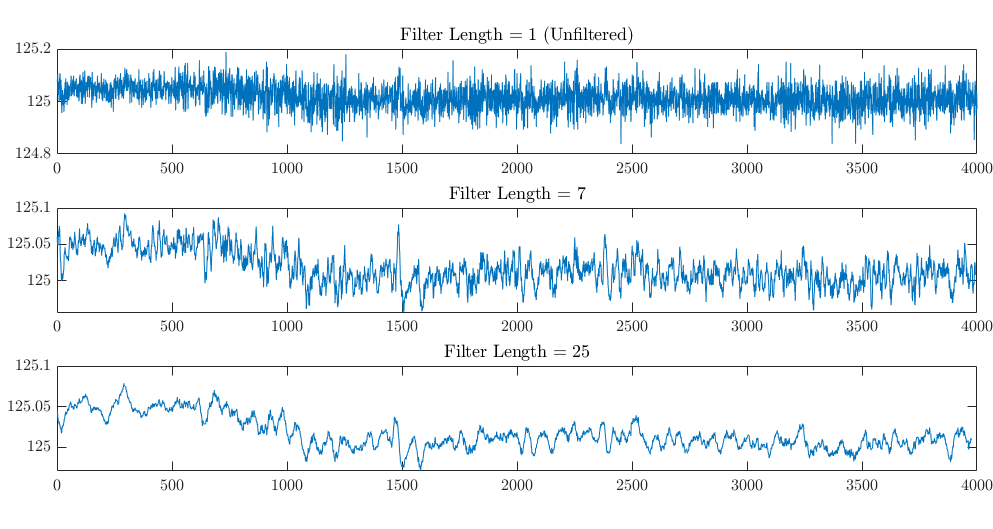
\includegraphics[width=0.99\textwidth]{figures/filter.png}
    \caption{Effect of sliding-window filter on the BFD output.}
    \label{fig:filter}
\end{figure}

\subsection{Filter Lengths on Output}
We implemented low-pass filters of various filter lengths in a sliding window fashion on the output signal. The effect of the sliding-window filter is visualized in Figure \ref{fig:filter}.\footnote{Selected from Week 1, Subbatch 19 in Tower 48 training data.} These experiments serve a two-fold purpose. Firstly, the training data contained a noisy signal for BFD. As a measure to avoid having the neural network train on the noise, the filter suppressed the high-frequency noise in the signal. In addition, we aimed to determine the impact of the filter on the model's ability to capture both low- and high- frequency process dynamics, as well as its generalizability. 

\subsection{Steady State Range Thresholds}
A component of our data pre-processing is selecting the range of values which we define as indicators of steady state behavior. Namely, the range selected is between the low and high BFD thresholds. However, the transient behaviors, which appear after recovering from a break, are essential to include in the model's training data. Refer to Figure \ref{fig:bfd_thresholds} for a comparison between two sets of thresholds. We attempted to widen said thresholds and include more transient behaviors of the plant, so to see the impact of exposing the neural network to more non-steady-state data on the robustness of the surrogate model. 

\begin{figure}[ht]
    \centering
    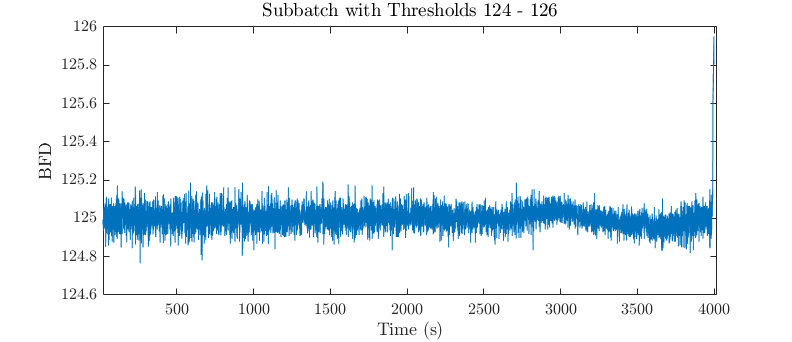
\includegraphics[width=\textwidth]{figures/thres_124126.png}
    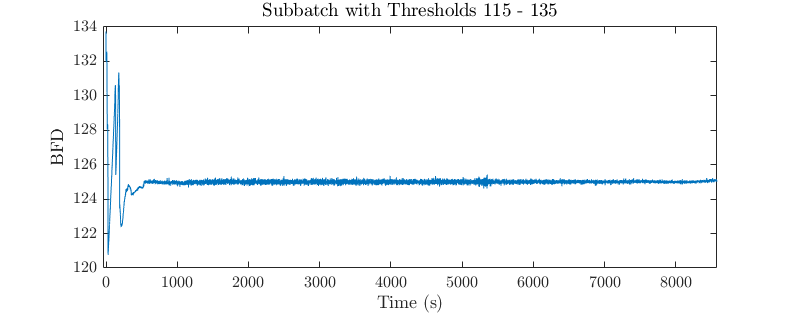
\includegraphics[width=\textwidth]{figures/thres_115135.png}
    \caption{Comparison between two sets of BFD thresholds in data pre-processing. Widened thresholds include more transient dynamics. }
    \label{fig:bfd_thresholds}
\end{figure}

\subsection{Long-Term Drift in Model Parameters}
Mechanical systems, especially those in continuous production, are susceptible to wear and tear over time and seasonal patterns. In developing this surrogate model of the fiber drawing plant, we were interested in whether the model parameters are time-varying in the long term, and by what extent if so. To examine the long-term patterns, we chose the best-performing model architecture from experiments mentioned above, validated it on each week of data, and examine the performance across all weeks. Separately, we also evaluated the performance of each week's model on all other weeks of data. 

\subsection{Model Specificity on Towers}

There were two fiber extrusion tower investigated, namely Tower 48 and Tower 51, with some process differences between the towers. We trained a deep LSTM network for each tower (hereinafter referred to as "Tower 48 model" and "Tower 51 model"), and we were interested in cross-validating the models' ability to predict the BFD output, i.e. using a model trained on one tower's data to predict on the other tower, and vice versa. From that outcome, we were to determine the necessity to separately train different models using production data measured in each tower. \\
\newline
The results of these experiments will be presented in Section \ref{ch:exp:results} below. 

\section{Training} \label{ch:exp:train}

We utilized 14 weeks worth of fiber drawing production data in each experiment. The training and testing datasets were partitioned by a 90:10 split on these data. All training experiments and analyses were performed using MATLAB R2021b. 

The training process involved tuning some hyperparameters to optimize for prediction accuracy. They are listed in Table \ref{tab:hyper_param}, most of which are obtained largely by trial and error. 

% explain init learning rate, learning rate schedules, (EXPLAINED IN CH2) how matlab implements it in drop period,  cite how it's effective

\begin{table}[b!]
    \centering
    \begin{tabular}{c c}
         Name & Value \\ \hline 
         Max epochs & 250\\ 
         Mini-batch size & 16\\ 
         Gradient Threshold & 10 \\ 
         Initial Learning Rate & 0.01 \\
         Learn Rate Drop Period & 100 \\ \hline
    \end{tabular}
    \caption{Hyperparameters for training the surrogate model.}
    \label{tab:hyper_param}
\end{table}

We began by comparing the ability of every architecture to learn and predict on unseen data.
All three architectures were trained for 250 epochs and the model with the lowest seen loss on the testing data was selected as output.
We present the testing losses of each of the architectures below.

\section{Metrics and Results} \label{ch:exp:results}

In evaluating the accuracy of one particular trained model, we used root-mean-square error (RMSE) between the measured BFD and predicted BFD as one of the metrics. However, the values of RMSE were used relatively, i.e. one particular RMSE has little meaning unless compared with RMSEs of other models. When examining the robustness of a surrogate model, we evaluated its performance by running inference on other inputs. All RMSEs are recorded in a \emph{cross-validation matrix} and patterns are observed. In addition, the power spectrum of the predicted dynamics is also evaluated. 

\subsection{Architecture Experiments}

\begin{table}[t!]
    \centering
    \begin{tabular}{r r}
         Architecture & RMSE \\ \hline
         Single Layer LSTM & 0.0817\\
         Single Layer BiLSTM & 0.0818\\
         Side by Side LSTM & 0.0817 \\
         Deep LSTM & 0.0824 \\ \hline
    \end{tabular}
    \caption{The four neural network architectures perform similarly on the RMSE metric. The single layer LSTM and side-by-side LSTM architectures appear to have the lowest RMSE, but have different output waveforms.}
    \label{tab:rmse_error}
\end{table}

The obtained RMSEs after training all four architectures are tabulated in Table \ref{tab:rmse_error}. Although the simple LSTM and side-by-side LSTM architectures got a similarly low RMSE, their output characteristics are very different. Evident in Fig. \ref{fig:prediction}, the single layer LSTM output is much closer to the real signal. The side-by-side LSTM network, however, was unable to accurately model the dynamics of BFD. Instead, it outputs a low-variance signal following the low frequency dynamics of BFD. Therefore, RMSE alone is not a sufficient metric to evaluate the performance of a black-box model; we are also interested in the model's performance as a function of frequency. A visual comparison of the power spectrum revealed that, the prediction agrees with the measured signal to a greater extent on the lower frequency range and the prediction performance slightly degrades at higher frequencies. The deep LSTM architecture performed the best, with its waveform closely following the real signal. It is thus selected as the architecture of choice for the following experiments performed. With the best-performing deep LSTM network, the prediction of tension error is illustrated in Figure \ref{fig:tension}. \footnote{Selected from Subbatch 32 of Tower 48 test data.}

\begin{figure}
    \centering
    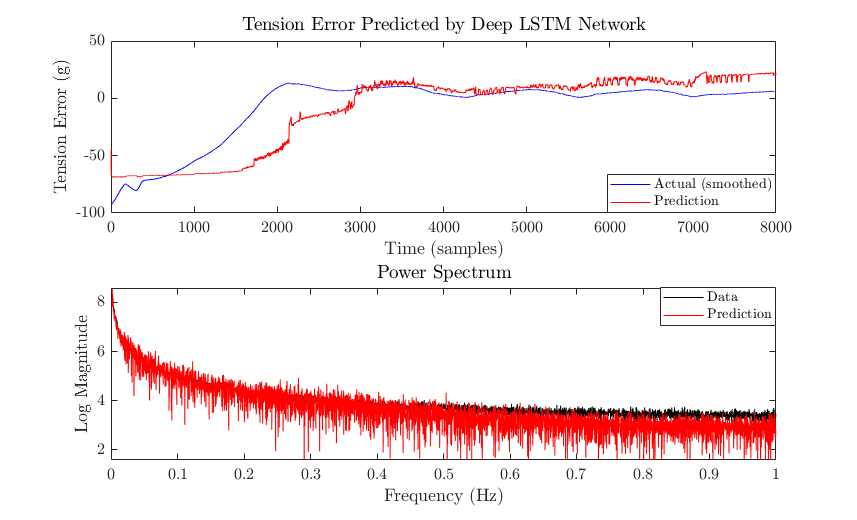
\includegraphics[width=\textwidth]{figures/tension.png}
    \caption{Deep LSTM model performance on predicting tension error. }
    \label{fig:tension}
\end{figure}

This result isn't surprising. Machine learning as a field is inherently experimental; the superior performance of the side-by-side architecture was proven in \cite{gonzalez} using synthetic data, whereas the real production data used in this study are completely different in nature. 

\subsection{Filter Lengths on Output}

% \begin{table}[h]

% \begin{tabular}{l|c c c c}
% \hline
%  & Data, no filter & Data, filter=3 & Data, filter=5 & Data, filter=7 \\ \hline
% Model, no filter    & 7.1883 & 7.9245 & 9.5703 & 11.2197 \\
% Model, filter=3     & 7.6234 & 8.1328 & 9.6085 & 11.1611 \\ 
% Model, filter=5     & 7.9734 & 8.1757 & 9.3822 & 10.7667 \\
% Model, filter=7     & 8.1633 & 8.3432 & 9.3241 & 10.5022 \\ \hline
% \end{tabular}

% \caption{Effect of Filter Lengths on Training Accuracy.}
% \label{tab:filter_len}
% \end{table}

\begin{figure}[h!]
    \centering
    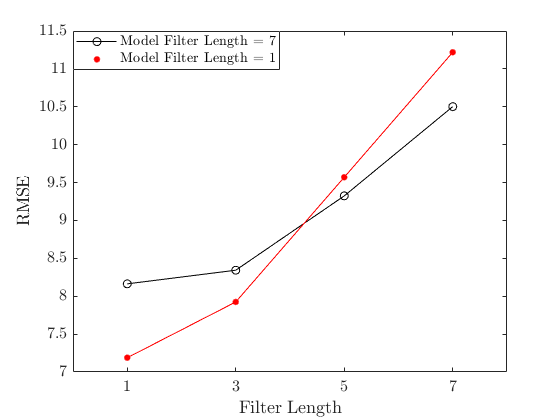
\includegraphics[width=0.75\textwidth]{figures/filter_length.png}
    \caption{Effect of filter length during training on model generalizability.}
    \label{fig:filter_len}
\end{figure}

%From the results from Table \ref{tab:filter_len} and the visualization in Figure \ref{fig:filter_len}, our 
The experiment outcomes shown in Figure \ref{fig:filter_len} suggest that a model trained on the unfiltered data (red curve) performed the best only on unfiltered or lightly filtered data, whereas a model trained on heavily filtered data (black curve) achieved mediocre performance for various filter lengths. With a more aggressive low-pass filter on the training data, the model learned the low-frequency components in all data, which makes it more robust in its prediction. Figure \ref{fig:filter_len_time_series} provides a comparison of model performances between both types of models in time- and frequency- domain.\footnote{Selected from Subbatches 43 and 243 of Tower 48 data, respectively.} The model trained on unfiltered data was able to predict the high-frequency dynamics in the BFD, whereas the one trained on filtered data only captured the low-frequency content in the BFD signal. 

\begin{figure}
    \centering
    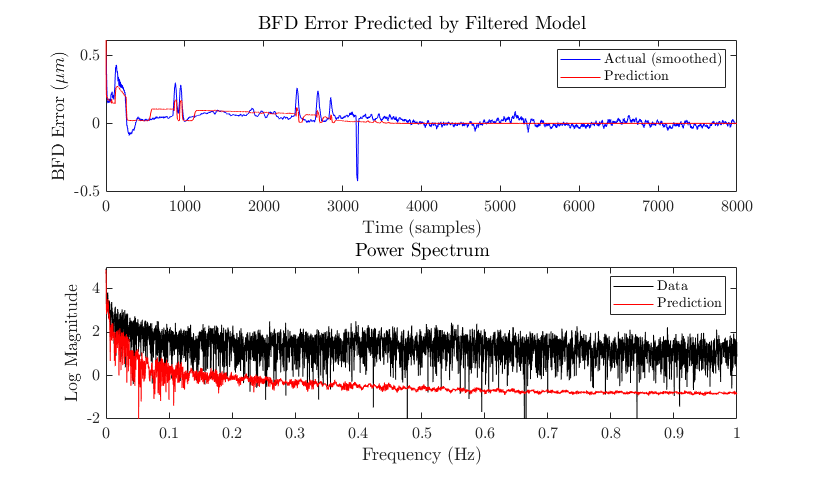
\includegraphics[width=\textwidth]{figures/filter_len_filtered.png}
    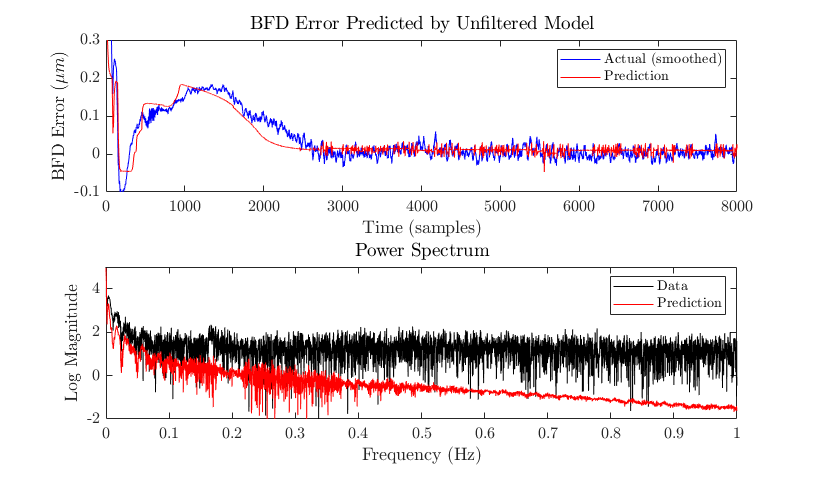
\includegraphics[width=\textwidth]{figures/filter_len_unfiltered.png}
    \caption{Comparison of model performances on BFD prediction using models trained on filtered (filter length of 7) and unfiltered (filter length of 1) data. The unfiltered training data give the model ability to recognize high-frequency dynamics.}
    \label{fig:filter_len_time_series}
\end{figure}

\begin{figure*}[ht!]
    \centering
    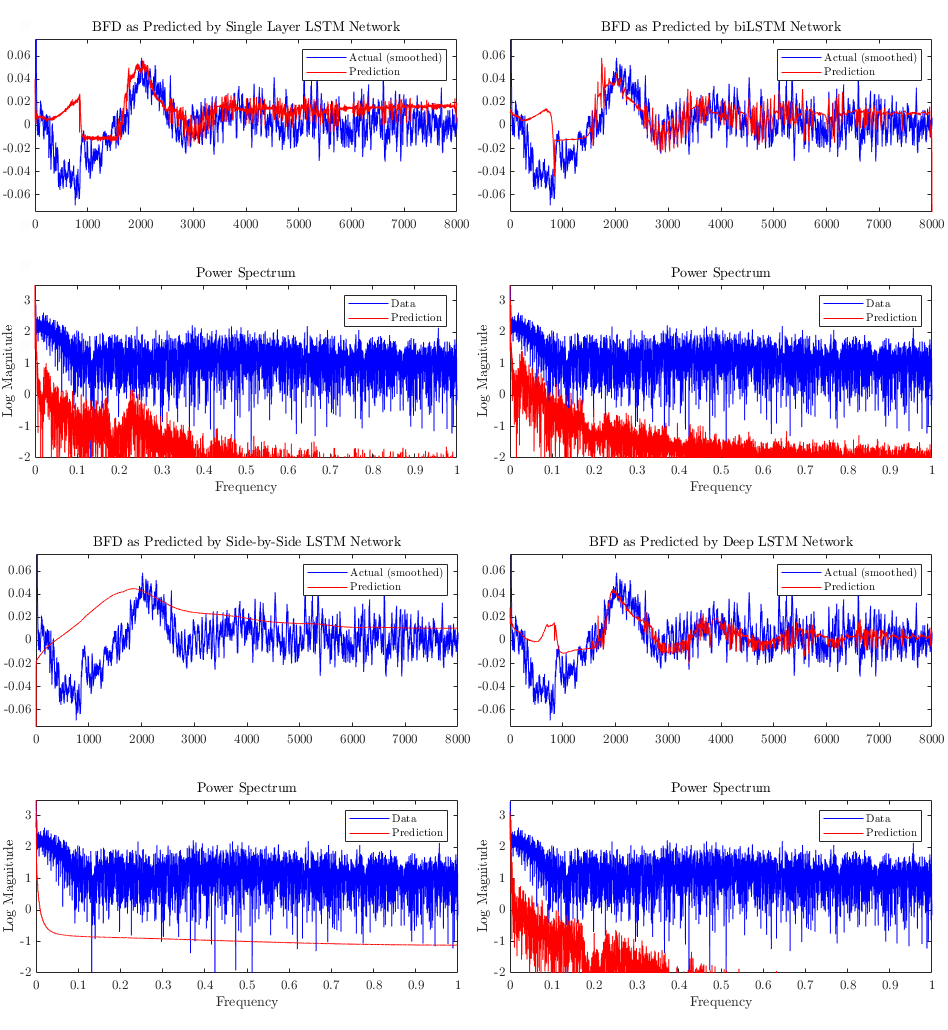
\includegraphics[width=\textwidth]{figures/combine_images.png}
    \caption{Mean-removed BFD as predicted by four network architectures.}
    \label{fig:prediction}
\end{figure*}

\subsection{Steady State Range Thresholds}

\begin{table}[ht!]
    \centering
        \begin{tabular}{|c|c|c|}
            \hline
            BFD Thresholds & RMSE & \makecell{RMSE on \\ 124-126 Data} \\ \hline
            124 - 126 & 0.0852 & 0.094\\
            123 - 127 & 0.0772 & 0.099\\
            122 - 128 & 0.0998 & 0.105\\
            121 - 129 & 0.1048 & 0.112\\
            120 - 130 & 0.1421 & 0.129\\
            119 - 131 & 0.1838 & 0.139\\
            118 - 132 & 0.2095 & 0.177\\
            117 - 133 & 0.2353 & 0.123\\
            116 - 134 & 0.3548 & 0.128\\
            115 - 135 & 0.2956 & 0.173\\ \hline
        \end{tabular}
        \caption{Effect of transient dynamics on RMSE and on model performance within region of interest.}
        \label{tab:thresholds}
\end{table}

Including more transient dynamics apparently compromises the machine learning model's ability to predict. This is represented by an increasing RMSE score across models when trained on data with varying amounts of transient dynamics. As shown in Table \ref{tab:thresholds}, the model trained on the least amount of transient dynamics was able to achieve the lowest RMSE, while all other models, trained on data with higher variance on the BFD, performed worse than the baseline. The modeling accuracy also did not benefit from including more transient dynamics on our data range of interest, 124 to 126 microns of BFD. This can be seen also in Table \ref{tab:thresholds}, where the model with the lowest RMSE on the data range of 124 to 126 is the model trained on said data range. 

\subsection{Long-Term Drift in Model Parameters}

\begin{figure}[ht!]
    \centering
    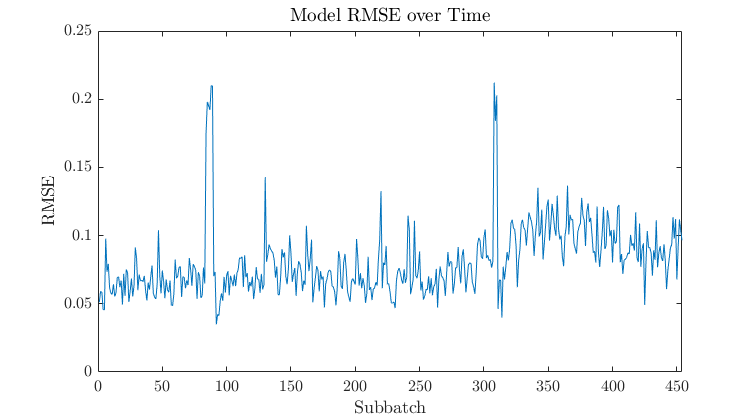
\includegraphics[width=\textwidth]{figures/drift.png}
    \caption{RMSE of the best-performing surrogate model over time.}
    \label{fig:drift}
\end{figure}

The deep LSTM neural network was shown to be the best-performing model in Section \ref{ch:exp:arch}. It was therefore chosen to perform inference on system output, namely the predicted BFD signal. The RMSEs of all subbatches of data (chronologically) are plotted in Figure \ref{fig:drift}. Note the few spikes in the RMSE; they correspond to the subbatches of shorter lengths than most other ones. This is because, to a certain extent, a higher data volume during the training of a model expands the convex hull of the training data and reduces the error in validation, enabling the model to generalize better. Future iterations of this study could normalize the subbatch length or the weigh the metric of RMSEs for comparable results. A similar effect of the subbatch length is also shown in the result of validating each week's model on all other weeks of data, particularly in Models 6 and 10 of Table \ref{tab:drift}.

\begin{table}[t!]
    \centering
    \resizebox{\textwidth}{!}{
    \begin{tabular}{c|c|c|c|c|c|c|c|c|c|c|c|c|c|c}
 & Week 1 & Week 2 & Week 3 & Week 4 & Week 5 & Week 6 & Week 7 & Week 8 & Week 9 & Week 10 & Week 11 & Week 12 & Week 13 & Week 14 \\ \hline
Model 1 & 2078 & 2635 & 250576 & 3056 & 2673 & 2049 & 2950 & 2101 & 2890 & 2811 & 3303 & 4858 & 3768 & 2887 \\
Model 2 & 2443 & 2527 & 18817 & 2718 & 2613 & 2327 & 2591 & 2383 & 2861 & 2514 & 3073 & 7939 & 11649 & 2786\\
Model 3 & 2333 & 6196 & 2064 & 3243 & 3066 & 2921 & 2599 & 2093 & 4417 & 2925 & 3854 & 3795 & 334879 & 3019\\
Model 4 & 2345 & 4691 & 2677 & 2414 & 2793 & 2386 & 8001 & 2473 & 2645 & 7739 & 8041 & 4616 & 5201 & 2522\\
Model 5 & 2924 & 4070 & 2698 & 3525 & 2678 & 3058 & 3754 & 2553 & 4424 & 3263 & 4329 & 4280 & 4376 & 3688\\
Model 6 & 4097 & 8823 & 1637684 & 12679 & 3399 & 2120 & 19559 & 355447 & 5007 & 15084 & 460871 & 2007124 & 6387426 & 2821549\\
Model 7 & 2743 & 3215 & 3003 & 2644 & 3014 & 2812 & 2357 & 2753 & 2881 & 2608 & 6908 & 3117 & 5141 & 2598\\
Model 8 & 6435 & 7538 & 25778 & 6158 & 3669 & 4607 & 4037 & 2327 & 7739 & 3364 & 9187 & 21440 & 7060 & 9731\\
Model 9 & 16709 & 10917 & 58923 & 3707 & 4242 & 3006 & 14607 & 54707 & 2588 & 14688 & 36115 & 89016 & 9550 & 3761\\
Model 10 & 55431 & 126472 & 76508 & 9518 & 26893 & 13851 & 2280 & 2006 & 61139 & 2134 & 105801 & 173357 & 57141 & 78577\\
Model 11 & 2313 & 2448 & 2365 & 2233 & 2344 & 2349 & 2269 & 2268 & 2478 & 2175 & 2665 & 2622 & 2453 & 2449\\
Model 12 & 2036 & 2559 & 2152 & 2348 & 2081 & 2320 & 2898 & 1826 & 2792 & 2824 & 2807 & 2526 & 2631 & 2320\\
Model 13 & 1814 & 2083 & 3598 & 2081 & 1862 & 1967 & 3063 & 1745 & 2241 & 2086 & 5645 & 8090 & 2247 & 2438\\
Model 14 & 2290 & 2847 & 2309 & 2493 & 2483 & 2603 & 3244 & 2095 & 2871 & 3374 & 3025 & 2799 & 2936 & 2408\\ \hline
    \end{tabular}
    }
    \caption{Cross-validation matrix of each week's trained model validating on all other weeks of data from Tower 48. }
    \label{tab:drift}
\end{table}

\subsection{Model Specificity on Towers}

\begin{figure}[ht!]
    \centering
    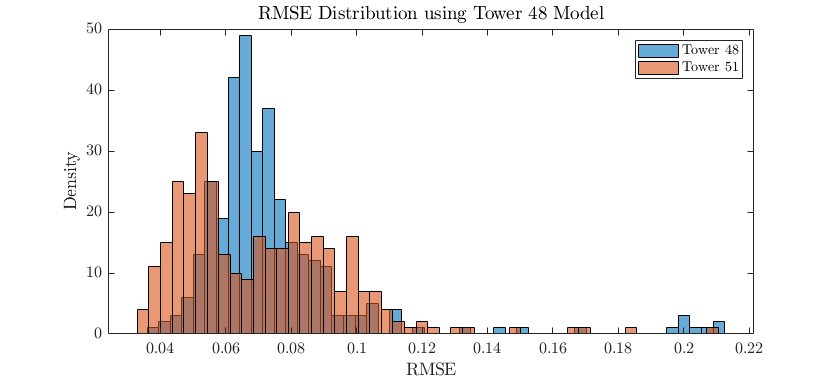
\includegraphics[width=\textwidth]{figures/model48_errors.png}
    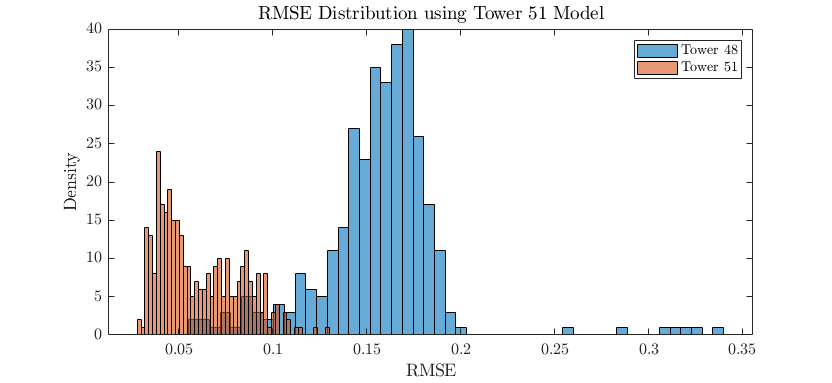
\includegraphics[width=\textwidth]{figures/model51_errors.png}
    \caption{Cross-validation of Tower 48 and Tower 51 models on each other's datasets.}
    \label{fig:tower_rmse}
\end{figure}

Figure \ref{fig:tower_rmse} offers a comparison of the RMSE distributions using the Tower 48 model and Tower 51 model, respectively. By running inference using the Tower 48 model on production data from each tower, we discovered that the RMSEs are similar in range, although the predictions on Tower 48 data are more consistent as compared to Tower 51 data, as shown by the lower variance in the histogram. The Tower 51 model demonstrated better performance on Tower 51 data only, and the Tower 48 model is more generalizable to Tower 51. 

\section{Discussion}

This chapter discussed an approach to model the optical fiber drawing process using LSTM networks. Using a deep LSTM neural network, we investigated the effects of filtering and inclusion of transient dynamics on model generalizability. Further fine-tuning of parameters could potentially lead to marginally better results, but a few limitations of this approach should be addressed. 

Firstly, each subbatch of data has a high variance due to variations in the production environment. The LSTM models may have slightly degraded performance when the validation data has amplitudes beyond the range seen within the training set \cite{lstm_amplitude}.

The process dynamics of fiber extrusion inherently does not have long-term memory. Instead, it is governed by a complicated set of governing differential equations that depends on the inputs, its current state, and finite-order differentials. It could be the case that the LSTM is erroneously finding long-term dependencies in the evolution of the BFD signal that do not actually exist. Further, memorizing past trajectories without learning the underlying dynamical structure has been proven ineffective in machine learning tasks involving nonlinear systems \cite{fu_et_al}. To address these problems, recommendations for further studies, which involve embedding the physical models into neural network models, are provided later in Section \ref{ch:concl:future_work}.